% THIS IS SIGPROC-SP.TEX - VERSION 3.1
% WORKS WITH V3.2SP OF ACM_PROC_ARTICLE-SP.CLS
% APRIL 2009
%
% It is an example file showing how to use the 'acm_proc_article-sp.cls' V3.2SP
% LaTeX2e document class file for Conference Proceedings submissions.
% ----------------------------------------------------------------------------------------------------------------
% This .tex file (and associated .cls V3.2SP) *DOES NOT* produce:
%       1) The Permission Statement
%       2) The Conference (location) Info information
%       3) The Copyright Line with ACM data
%       4) Page numbering
% ---------------------------------------------------------------------------------------------------------------
% It is an example which *does* use the .bib file (from which the .bbl file
% is produced).
% REMEMBER HOWEVER: After having produced the .bbl file,
% and prior to final submission,
% you need to 'insert'  your .bbl file into your source .tex file so as to provide
% ONE 'self-contained' source file.
%
% Questions regarding SIGS should be sent to
% Adrienne Griscti ---> griscti@acm.org
%
% Questions/suggestions regarding the guidelines, .tex and .cls files, etc. to
% Gerald Murray ---> murray@hq.acm.org
%
% For tracking purposes - this is V3.1SP - APRIL 2009

\documentclass{acm_proc_article-sp}

\usepackage{amsmath}
\usepackage{algorithm}
\usepackage{dsfont}
\usepackage[noend]{algpseudocode}
\usepackage{pbox}

\begin{document}

\title{toMEto: a Networks-based Approach to Recipe Recommendation}
\subtitle{CS145}


\makeatletter
\def\BState{\State\hskip-\ALG@thistlm}
\makeatother


\numberofauthors{4} 
\author{
\alignauthor
Albert Ge\\
       \affaddr{California Institute of Technology}\\
       \affaddr{Pasadena, CA}\\
       \email{age@caltech.edu}
\alignauthor
Matthew Jin\\
       \affaddr{California Institute of Technology}\\
       \affaddr{Pasadena, CA}\\
       \email{mjin@caltech.edu}
\and % go to new row
\alignauthor
Jonathan Joo\\
       \affaddr{California Institute of Technology}\\
       \affaddr{Pasadena, CA}\\
       \email{jjoo@caltech.edu}
\alignauthor
Boyu (Charlie) Tong\\
       \affaddr{California Institute of Technology}\\
       \affaddr{Pasadena, CA}\\
       \email{bttong@caltech.edu}
}

\date{05 June 2016}


\maketitle
\begin{abstract}
toMEto is a web-based application that suggests ingredients to supplement existing recipes. We develop and evaluate several network based algorithms, packaging the suggestions under an intuitive and friendly user interface. 
\end{abstract}

% A category with the (minimum) three required fields
%\category{H.4}{Information Systems Applications}{Miscellaneous}
%A category including the fourth, optional field follows...
%\category{D.2.8}{Software Engineering}{Metrics}[complexity measures, performance measures]

%\terms{Theory}

%\keywords{ACM proceedings, \LaTeX, text tagging} % NOT required for Proceedings

\section{Introduction}
Traditionally, cooking involves a combination of technical skills and creativity. While technical skills can only be improved through time and practice, we believed that the creative aspect of cooking could be improved through utilizing the wealth of existing recipes available online. There are a variety of web and mobile applications that mostly function as a database for recipes, and allow users to quickly search to recipes pertaining to their desires. There are also more advanced applications that devote specifically to \textit{food pairings}; websites such as \texttt{foodpairing.com} allow users to experiment with different ingredients and rate their synergy by examining the flavor network. On another hand, \texttt{yummly.com} will recommend new recipes based on a variety of selection filters, such as allergies or diets. 

The purpose of this project is to be able to blend the two and suggest individual ingredients, as opposed to entire recipes, using the concept of food pairings found through an ingredient network. Thus, through construction of a network using this information, toMEto offers unique suggestions to create interesting new twists on already successful recipes. Having these suggestions available alongside a recipe allows toMEto to inspire new forms of cooking styles, and improves the creative cooking experience for beginners and advanced chefs alike. With a simple, intuitive user interface, along with a rich database of recipe information, toMEto allows for a streamlined recipe lookup experience, with the added functionality of optimized suggestions. 

The rest of the paper is organized as follows. Section 2 contains details on data scraping and other preprocessing steps. Section 3 describes the various algorithms considered. Section 4 covers the app's web design while Section 5 covers the backend. Section 6 concludes our paper. 


\subsection{Related Work}

There have been a select number of papers discussing analysis of food and ingredient networks. In the literature, there are two common food networks that subject to network analysis. The first is a \textit{co-occurrence network}, which relates ingredients by how often they appear together in user-defined recipes. The other is a \textit{flavor compound network}, which relates ingredients by how similar their chemical composition is. Throughout this paper we will refer to the co-occurrence network as the \textit{ingredient network}, and the flavor compounds network as the \textit{flavor network.}
Teng et al.~\cite{recommend} describes the goal of being able to recommend entire recipes, using recipe suggestions made by examining communities of a co-occurrence network, to predict the success of a particular recipe's rating. 

Another paper by Ahn et al.~\cite{pairings} compares the differences in cuisine by instead looking at a flavor-compounds network, and making general statements about the co-occurrence of ingredients by their chemical composition. They discovered that Asian recipes tend to have ingredients with different compounds, whereas Western cuisines have ingredients with like compounds. 

Still other research is ongoing, some building upon the relevance of flavor compounds 
in regional cuisines~\cite{zhu2013geography},~\cite{jain2015analysis}, and others attempt to implement these ideas to help users make suggestions about healthy food choices~\cite{Geleijnse}.

Within this web of research, we discovered a potential niche for recommending individual \textit{ingredients}, as opposed to entire recipes. This combines both the practical application of current research on food networks, as well as the theory behind identifying ingredients that are compatible with each other.


\section{Data Processing}

\subsection{Data source}
Our application's source of data are the online recipe websites New York Times (NYT) Cooking and AllRecipes.com. We gained over 13,000 and 52,000 recipes by crawling and scraping these two websites respectively. This was done by a script written in \texttt{scraper.py}. 

\subsection{Initial parsing}
Our application only requires the title, ingredients, and body of each recipe, so we extracted this data from each webpage using a simple script written in \texttt{parser.py}.

However, this extracted data was not in a clean format that our algorithms could easily use. For example, ingredients were often combined with quantifiers and other adjectives:
\begin{itemize}
       \item {\em medium-size russet potato, about 10 ounces, peeled and diced}
       \item {\em shrimp, shelled and cut into bite-sized pieces}
       \item {\em kale, stemmed, rinsed and coarsely chopped to make 6 cups}
\end{itemize}
These ingredients would only occur maybe once or twice in the entire dataset, resulting in many ``rare'' ingredients. In the NYT dataset (12402 unique ingredients), approximately 70\% of the unique ingredients occurred only once, and 90\% occurred less than 10 times. We realized this resulted in suboptimal performance, as these ingredients would not be counted correctly in the ingredient network and many edges would not exist in the network.

\subsection{Mapping}
To fix this, we developed a script in \texttt{nyt\_mapper.py} to find these ``rare'' ingredients and map them to their root ingredient. For the example ingredients from above, we generated the mappings:
\begin{itemize}
       \item {\em medium-size russet potato, about 10 ounces, peeled and diced} $\to$ {\em potato}
       \item {\em shrimp, shelled and cut into bite-sized pieces} $\to$ {\em shrimps}
       \item {\em kale, stemmed, rinsed and coarsely chopped to make 6 cups} $\to$ {\em kale}
\end{itemize}
The script attempts to extract the root ingredient for each entry by combining several strategies. For example, some strategies that we use are:
\begin{itemize}
       \item Removing parenthetical tokens 
       \begin{itemize}
              \item {\em vanilla extract (to taste)} $\to$ {\em vanilla extract}
       \end{itemize}
       \item Removing comma separated descriptors 
       \begin{itemize}
              \item {\em honey, preferably wildflower} $\to$ {\em honey}
       \end{itemize}
       \item Picking the best of two ingredients separated by `or' 
       \begin{itemize}
              \item {\em sriracha or other hot sauce} $\to$ {\em sriracha}
       \end{itemize}
       \item Finding a sole `top' ingredient name 
       \begin{itemize}
              \item {\em coarsely grated carrot} $\to$ {\em carrots}
       \end{itemize}
\end{itemize}
Using the mappings generated by \texttt{nyt\_mapper.py}, we reduced the unique ingredient count by 75\%. This resulted in a much more densely connected network, and more accuracy in recommendations.

\subsection{Supplementing with AllRecipes data}
We initially focused our application on the NYT dataset due to the relatively cleaner data and ingredients list. Once our basic algorithms were up and running on this dataset, we moved to supplement it with the much larger AllRecipes dataset (52,000 recipes). We reasoned that this would further improve the ingredient network by providing a more accurate count of ingredient frequencies. We also expected it to introduce new connections (and thus new, creative suggestions), since there may be recipes and foods that are not found in the NYT dataset.

As our application does recommendations only for NYT recipes, we modified our approach to processing the AllRecipes data accordingly. Again, we wrote a mapping script in \texttt{allrecipes\_mapper.py}, but instead of mapping to only the root ingredients, the script also attempted to map to the top ingredients in the NYT dataset. This was important because our goal ultimately was to develop an ingredient network for the NYT dataset, and we did not want the ingredients of the AllRecipes dataset to be disjoint in any way. 

The AllRecipes mapper employed many of the same techniques as the NYT mapper, with some additional strategies. The recipes from the AllRecipes websites list the ingredients with numbers and quantifiers, for example:
\begin{itemize}
       \item {\em 1 pound ground beef}
       \item {\em 1/2 teaspoon black pepper}
       \item {\em 1 (25 ounce) package frozen cheese ravioli}
\end{itemize}
Thus, we added filters that removed numerical digits from the raw ingredient name and also searched for and removed quantifiers such as ``pound'', ``teaspoon'', or ``ounce''. To map the ingredients to the NYT ingredients, we took a set of the most common NYT ingredients and searched for corresponding tokens in the AllRecipes ingredients. If there was a 1-to-1 matching, then we considered it a mapping.

Combining both datasets resulted in a network with 7339 unique ingredients. Of these, we selected the top 1000 which approximately corresponded to the set of ingredients with at least 10 occurrences. For several of our algorithms, we restricted the recommendations to be from within this ``top set'' in order to have meaningful suggestions.



\section{Algorithm Design and Analysis}

The primary application of algorithm design resides in ingredient recommendation to the user. These algorithms were implemented in a collection of files with the pattern \texttt{analyzer\_*.py}, and each file corresponds to a different algorithm (as we enumerate below). We reserve the majority of this section to understanding the different frameworks we tried for the \textit{complement} method, which is a method that takes in a particular recipe ID, and suggests up to ten ingredients that the user could potentially add. 

Before we do so, however, we first introduce some common terminology to be used throughout the text:
\begin{enumerate}
	\item \textit{w(x,y)} describes the weight of the edge between two ingredients. We define the weight
	of an edge as the co-occurrence of two ingredients; that is, how many times the two ingredients 
	appear in the same recipe. 
	\item \textit{graph} is the entire ingredient network.
	\item \textit{peripheral ingredient} describes those ingredients that are not part of a recipe, but have at least one edge (with nonzero weight) to an ingredient in the recipe (Fig. 1). Formally, this is described as
	\[\{k : \text{k} \in \text{adjacent neighbors of recipe} \wedge k \notin \text{recipe}\}
	\]
	\item \textit{compatibility score} is a score computed (using different metrics) that
	is used to rate each ingredient suggestion. An ingredient with high ``compatibility''
	with another suggests that the pair are commonly used together, and therefore
	would be a good fit for the recipe.
\end{enumerate}


\begin{figure}
	\centering
	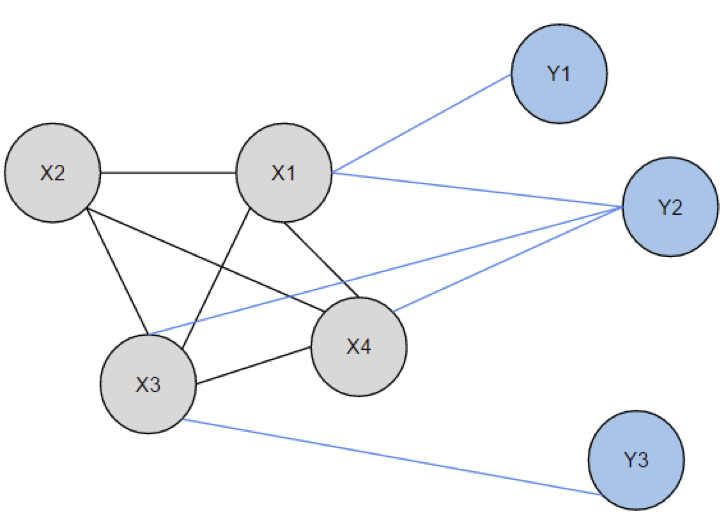
\includegraphics[width=5cm]{peripheral}
	\caption{Peripheral ingredients. Nodes denoted in gray are part of recipe $X$, while ingredients in blue
	are peripheral ingredients with connections to some of the recipe ingredients.}
\end{figure}


There are two primary schools of thought when designing an appropriate algorithm for recipe recommendation - using degree centrality measures, versus using pointwise mutual information (PMI). Here we enumerate in detail the algorithms. \\
First, we discuss the algorithm that uses degree centrality. We apply degree centrality toward compatibility scores of ingredients.

\begin{enumerate}
	\item Degree Centrality (Algorithm 1). 
	The key aspect of this algorithm was to compute a compatibility score 
	of an ingredient by summing over the all its connections with ingredients in the recipe. 
	For two ingredients $(a,b)$, we compute the weight of its connection by $w(a,b)$ by 
	counting the number of occurrences $a,b$ appear together in the same recipe. 
	Each connection is normalized by dividing by the highest weighted number of connections of 
	the two ingredients; this helps prevent other high-frequency ingredients from
	dominating the recommendation. To compute the the weighted number of connections of 
	an ingredient $a$, we sum the weights over all the connections with its neighbors: $\sum_{b \in N(a)} w(a,b)$.
	\\
	 Formally, we write, for a pair of ingredients $(i, k)$
	with $i$ being a recipe ingredient and $k$ a peripheral ingredient,
	\[score = \sum_{i \in recipe} \min(\frac{w(i,k)}{degree(i)},\frac{w(i,k)}{degree(k)})
	\]

\end{enumerate}

This algorithm was the first variant that we attempted on ingredient recommendation. First, we obtain a list of 
	all peripheral ingredients of a particular recipe. 
	 Here, we exclude the top ten ingredients
	as part of our search. The idea was to exclude potentially obvious or very
	similar ingredients from our search - we wanted to suggest something that would 
	introduce variability to our suggestions, rather than recommend the same
	high-frequency ingredients. Additionally, we must check if ingredients
	exist in the network, as our data processing eliminates certain ingredients
	from the graph but doesn't eliminate them from the recipes themselves.

\begin{algorithm}
\caption{Degree Centrality algorithm}
\begin{algorithmic}[1]
  \Function{naive}{$recipeID$}
  	\State Let $recipe$ = recipe with ID $recipeID$
    \State Let $top10$ = ten ingredients with highest weighted number of connections
    \State Let d = dictionary to contain all ingredients and their compatibility score
    \For{$i$ in ingredients of $recipe$}
    	\If {$i$ in graph and $i$ not in $top10$}
    		\For{peripheral ingredient $k$}
    			\State{$d[k] = d[k] + \min(\frac{w(i,k)}{degree(i)},\frac{w(i,k)}{degree(k)})$}
    		\EndFor
    	\EndIf
    \EndFor
    \Return 10 ingredients from $d$ with highest compatibility score
   \EndFunction

\end{algorithmic}
\end{algorithm}

Since this algorithm takes an arbitrary standard of excluding the top ten ingredients from recommendation, this was initially seen as a naive algorithm for recipe recommendation. Hence, we turned to a much more extensive analysis of using
PMI as the basis of our algorithms. The general formula of PMI, between two ingredients $a,b$ is given by:
\[
	\log \frac{p(a,b)}{p(a)p(b)}
\]
where $p(a)$ is defined as $\frac{\text{number of occurrences of a}}{\|graph\|}$. Intuitively, this value between
two ingredients describes how likely two ingredients are to appear together in the graph. Two ingredients with very few connections could still have a high value according to this metric, if they appear together more often than they do not. Thus it was thought that this metric captures ingredient pairings much better, as now there isn't any need to remove the most frequent ingredients.

As in degree centrality, we use PMI mainly for computing compatibility scores of ingredients.

Here we enumerate the algorithms using PMI:
\begin{enumerate}
	\item Normalized PMI. After computing a score using PMI, normalize the value by the weighted number
	of connections. This algorithm is the exact same as in Algorithm 1, only the weight $w(a,b)$ is subsituted for $PMI(a,b)$. This was mostly meant to compare directly with the the degree centrality algorithm.
	\item Generalized PMI (Algorithm 2). This is an extension to the pairwise PMI score, and generalizes it PMI between more than 2 ingredients. For an $n$-tuple of ingredients in the recipe, we compute sum of all their weighted connections with each other $\sum_{a, a' \in tuple} w(a,a')$. We then find the tuple whose
	sum of weights is the greatest - this captures the ingredients that are seen together most often in recipes,
	and gives us a sense of the ``essential'' ingredients in the recipe. Then, using these essential ingredients,
	we can compute a generalized PMI score for each peripheral ingredient that has connections to all of
	these essential ingredients, which is given by 
	\[
		PMI(tuple) = \log \frac{p(x \in tuple)}{\prod_{x \in tuple}p(x)}
	\]
	In practice, we found that letting $n = 3$ for determining the size of our tuple was best, as
	it as large as we could get without too many division by zero errors. 
       \item Weighted PMI (Algorithm 3). This weights an ingredient's PMI score by the number of edges that exist between
       itself and ingredients of the recipe. Formally, for a peripheral ingredient $b$ we describe this as
       \[
              (\sum_{a \in recipe} \mathds{1}_{(a, b) \in graph})(\sum_{a \in recipe} PMI(a, b))
       \]
       Thus, for each connection to an ingredient in the recipe, we increase the weight factor by 1. Intuitively, this assigns more importance to peripheral ingredients
       that pairs well with many of the recipe's ingredients. 
	\item Minimax PMI. This algorithm was meant to consider safe suggestions; that is, recommending peripheral ingredients that would be compatible with all recipe ingredients, instead of ingredients
	that would work very well with some and not at all with others in the recipe. To do this,
	for a peripheral ingredient $b$ we computed $\min_{a \in recipe} PMI(a,b)$, and then 
	returned the ingredients with the highest min values. This way, we could rule out ingredients
	that would never pair well with at least one recipe ingredient.
\end{enumerate}

  \begin{algorithm}
   \caption{Generalized PMI algorithm}
    \begin{algorithmic}
      \Function{genPMI}{$recipeID$}
       \State Let $recipe$ = recipe with ID $recipeID$
        \State Let $top10$ = ten ingredients with highest weighted number of connections
        \State Let d = dictionary to contain all ingredients and their compatibility score
       \State{$bestMatch=\max_{(a,b,c) \in recipe} w(a, b) + w(b,c) + w(a,c)$ }
       \State{$tuple=\text{argmax}_{(a,b,c) \in recipe} w(a, b) + w(b,c) + w(a,c)$ }
        \For{$i$ in ingredients of $tuple$}
              \For{peripheral ingredient $k$ and $a, b, c \in N(k)$}
                     \State{$d[k] = PMI(k, tuple)$}
              \EndFor
        \EndFor
        \Return 10 ingredients from $d$ with highest compatibility score
       \EndFunction

\end{algorithmic}
\end{algorithm}

  \begin{algorithm}
   \caption{Weighted PMI algorithm}
    \begin{algorithmic}
      \Function{wPMI}{$recipeID$}
      	\State Let $recipe$ = recipe with ID $recipeID$
        \State Let $top10$ = ten ingredients with highest weighted number of connections
        \State Let d = dictionary to contain all ingredients and their compatibility score
        \For{$i$ in ingredients of $recipe$}
        	\If {$i$ in graph}
        		\For{peripheral ingredient $k$}
        			\State{$d[k] = d[k] + \min( \frac{PMI(a,b)}{degree(b)}, \frac{PMI(a,b)}{degree(a)})$}
        			\State{$count[k] = count[k] + 1$}
        		\EndFor
        	\EndIf
        \EndFor
        \For{ingredient in $d$}
        	$d[k] = d[k] \cdot count[k]$
        \EndFor
        \Return 10 ingredients from $d$ with highest compatibility score
       \EndFunction

\end{algorithmic}
\end{algorithm}


Furthermore, we compared these algorithms using an objective test. First, we separated the dataset into two parts. The first part, the part used for ``learning'', consisted of 70\% of the dataset, and the second part, the part used for testing, consisted of 30\% of the dataset. The separation of this dataset was done randomly to ensure that there was no bias in the learning and testing sets. (For example, we wanted to avoid a case where all the baked goods ended up in the learning set, skewing results.) Then, we applied our algorithms on the the learning set, and tested their recommendations on the testing set, with each recipe having one ingredient removed. When removing one ingredient from each testing recipe, we chose an ingredient that was a top 1000 ingredient, to make sure it had a chance at being recommended. The algorithms were evaluated on their ability to recover the one missing ingredient. This gave us an objective and fair test between the algorithms, and we found that the \textit{weighted PMI algorithm} was the most successful. 

However, it was only able to recover the missing ingredient about 20\% of the time. While this indicates some failure with our algorithms, it is really a misalignment of objectives. Our algorithms try to recommend a novel ingredient to spice up a dish, whereas the algorithm analyzer awards points for recovering a missing ingredient. These use cases, albeit similar, are clearly different. It is quite difficult to have an objective test that evaluates how good the algorithms are.




\section{Web Design}

Web design was done using a combination of HTML, CSS, JavaScript, and Python. HTML was used to create the content for display on the page, and CSS was used to style this content. JavaScript was also used for animations and general User Interface tweaks to make browsing the site intuitive and smooth. Finally, Python was utilized as an interface between the back-end and the front-end. Through the usage of Python's Flask framework, it was possible to integrate the back-end algorithms with displaying the relevant computed information on the front-end. In other words, our module app.py imported modules from the back-end, while also using this information to fill in the HTML templates based on search queries, etc. given by a user in the front end. 

The primary focus on the front end was to develop a site that is intuitive and self-explanatory, while also featuring only the information that is needed the most. Thus, the landing page has the following design:

\begin{figure}[H]
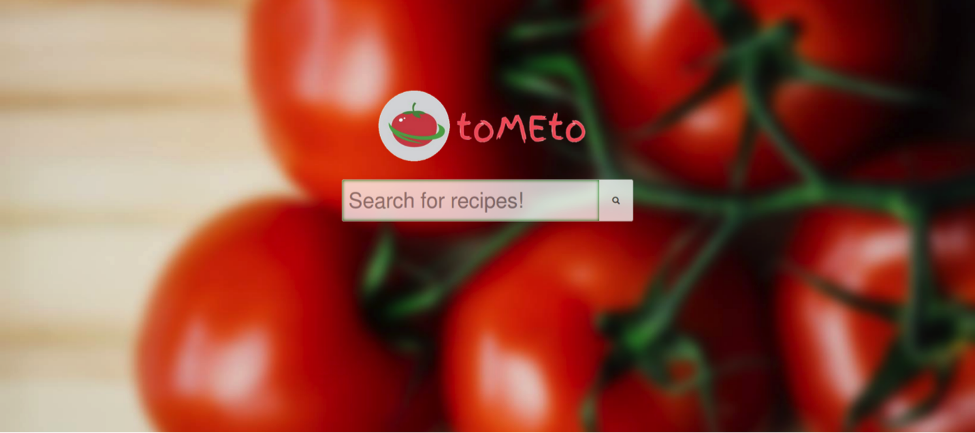
\includegraphics[scale=0.5]{p1.png}
\caption{Landing page for toMEto.}
\end{figure}


Upon searching for a recipe, a loading bar appears, and once recipe information is obtained, tiles fade in. These tiles offer an image of the recipe to be prepared, with the recipe title overlaid on top. This can be seen below:
\begin{figure}[H]
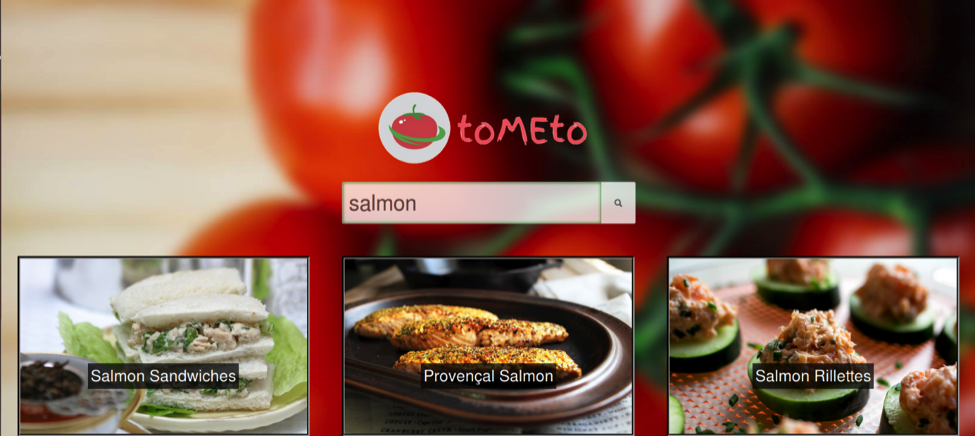
\includegraphics[scale=0.5]{p2.png}
\caption{Tiles, each with a recipe related to the search input.}
\end{figure}
Upon clicking a recipe, a modal popup appears, which lists both the recipe itself as well as toMEto's recommended ingredients, as can be seen in the below image:
\begin{figure}[H]
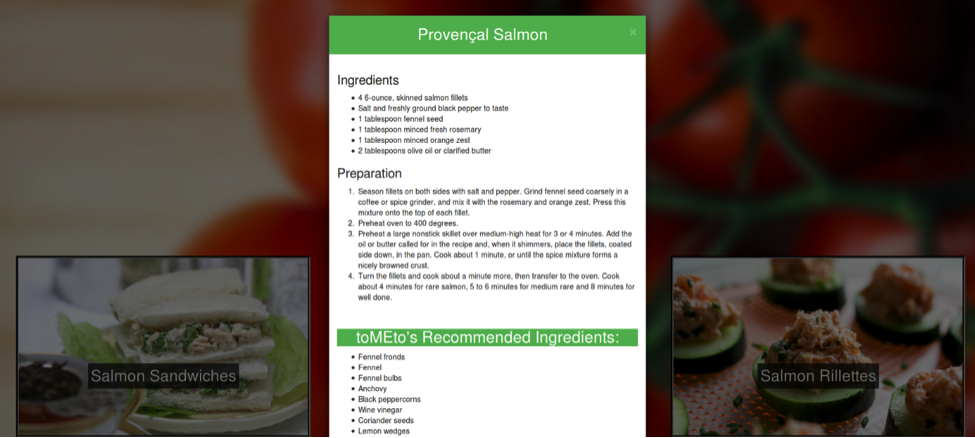
\includegraphics[scale=0.5]{p3.png}
\caption{The resulting popup from clicking on an image, with the recipe and our recommended ingredients.}
\end{figure}
Much of the front-end was designed to be easily updated and maintained, and thus small UI tweaks, such as background images, color schemes, etc. are easily changeable by editing the HTML and/or CSS files. The front-end utilizes mainly three different HTML templates:
\begin{itemize}
\item \texttt{simplesearch.html}
\item \texttt{simplesearch\_searched.html} 
\item \texttt{no\_results.html}
\end{itemize}
\texttt{simplesearch.html} is simply the html for the landing page, before any queries are entered. Then, once a search query is entered, app.py directs this information to the backend, which then generates information which is supplied to the \texttt{simplesearch\_searched.html} template. The user is also redirected to this template, which includes the tiles, modal popup information, etc. Furthermore, if a search is entered into \texttt{simplesearch\_searched.html}, this also refreshes the \texttt{simplesearch\_searched.html} template, utilizing the new information. Finally, \texttt{no\_results.html} is used as a template to be redirected to when the query entered into \texttt{simplesearch.html} or \texttt{simplesearch\_searched.html} does not contain any results. As a note, a user will be redirected to \texttt{simplesearch.html} upon clicking the toMEto logo.

\begin{figure}
\centering
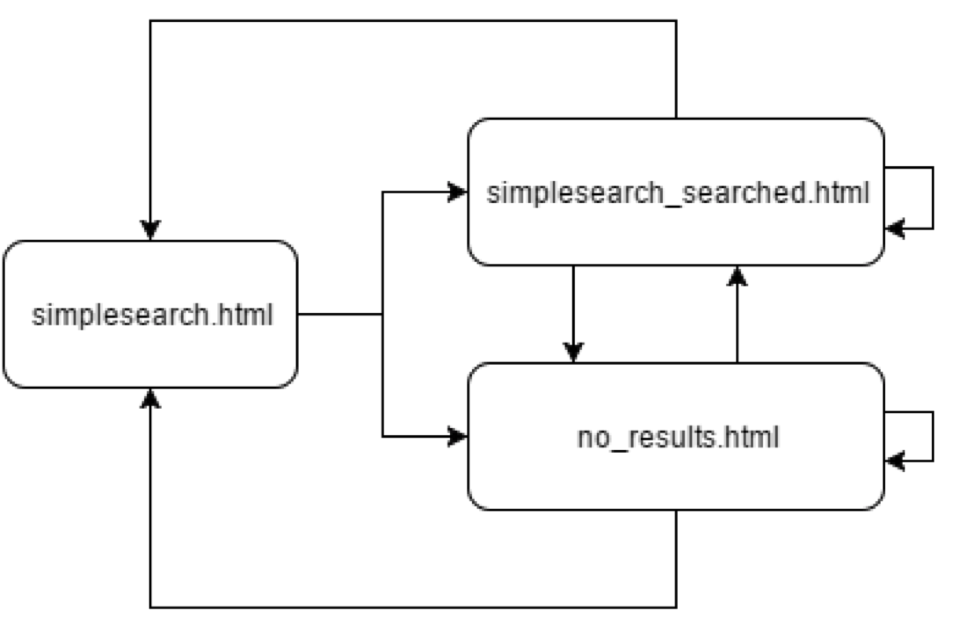
\includegraphics[scale=0.5]{p4.png}
\caption{Diagram of front-end architecture. \texttt{simplesearch.html} is the landing page of the website,
and after a search query, the webpage will then transition into either \texttt{simplesearch\_searched.html} if there are search results, or \texttt{no\_results.html} if there are no results. Additional search queries will just redirect into the corresponding HTML page.}
\end{figure}


\section{Backend Architecture}

\begin{figure*}[t]
	\centering
	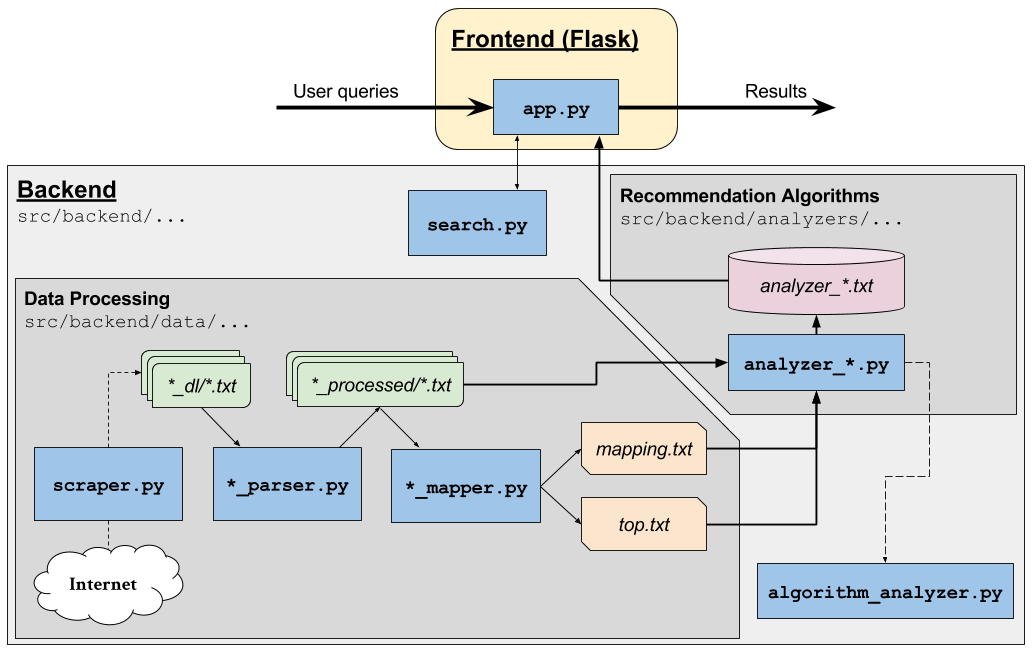
\includegraphics[width=\textwidth]{architecture}
	\caption{Schematic of the architectural design.}
	\label{fig:}
\end{figure*}

\subsection{Integration with Frontend}
A diagram of our backend architecture is described in Figure 6. We first launch the service by calling \texttt{app.py}, as well as invoking the appropriate \texttt{analyzer\_*.py} program whose algorithm we wish to display. Shortly after, the landing page for toMEto is brought up. The user then can enter a search query,
which gets passed through \texttt{app.py}, and then \texttt{search.py} in the backend. The relevant
recipes are returned back through \texttt{app.py}, which then looks through a text file \texttt{analyzer\_*.txt} to find our recommended ingredients for the returned recipes. Finally, these are displayed to the user 
 as a webpage.

\subsection{Backend processing}
As described in Section 2 of this paper, we use the following
modules to extract and obtain relevant recipe information, to be fed to \texttt{app.py}.
\begin{enumerate}
	\item First, use module \texttt{scraper.py} to scrape recipes from the Internet
and store raw data in a folder \texttt{dl/}. 
	\item Then, we employ \texttt{parser.py} to parse out the relevant recipe data and store the recipes in a folder \texttt{processed/}. 
	\item Run \texttt{mapper.py} to create two files: \texttt{mapping.txt}, which maps
		similar ingredients to the same ingredient, and \texttt{top.txt}, which lists
		the ~1000 most common ingredients.
	\item These are fed into the \texttt{analyzer\_*.py} files, which produce the ingredient networks
		and run the relevant algorithms described in Section 3. These functions will run
		the algorithm on each recipe obtain from NYTimes Cooking, and save all the results 
		in the corresponding \texttt{analyzer\_*.txt} files.
\end{enumerate}

\section{Conclusions and Future Work}

The final result of our project is a web based application that suggests supplementary ingredients to existing recipes. The novel part of our application lies in our algorithms, where we use purely network metrics to rank ingredient suggestions. The generalized PMI algorithms had the most success in providing solid, consistent recommendations.

There are also several features that could be implemented to further improve toMEto. At the moment, recipes are found using a database. Allowing the user to specify his own recipe with a set of ingredients and then recommending supplementary ingredients would be a very useful feature. This would not be very difficult to implement with our current architecture. The one challenge here is restricting or preprocessing user inputs to match those in the existing ingredient network.

We could parse the dataset and classify them, allowing users to get suggestions for a certain type of recipe. For example, some classifications could be how the recipe is cooked (baked, fried, etc.) or the type of cuisune. Then, suggestions that appear will be restricted to the type of recipe the user is interested in.

Furthermore, we could allow user personalization. Allow the user to upvote or downvote suggestions, and use machine learning techniques to determine what kind of additions the user likes. This would require new algorithms to supplement our existing network algorithms.


%%%%%%%%%%%%%%%%%%%%%%%%%%%%%%%%%%%
%%%% Compiling Instructions %%%%%%%
% pdflatex report.tex
% bibtex report
% pdflatex report.tex
% 
% You have to compile twice to get the references to show up

\bibliographystyle{abbrv}
\bibliography{report}

%\balancecolumns 


\clearpage
\onecolumn
\section*{Appendix A: Larger versions of Figures 2-4}
\vspace{3mm} %3mm vertical space

\begin{figure}[H]
\centering
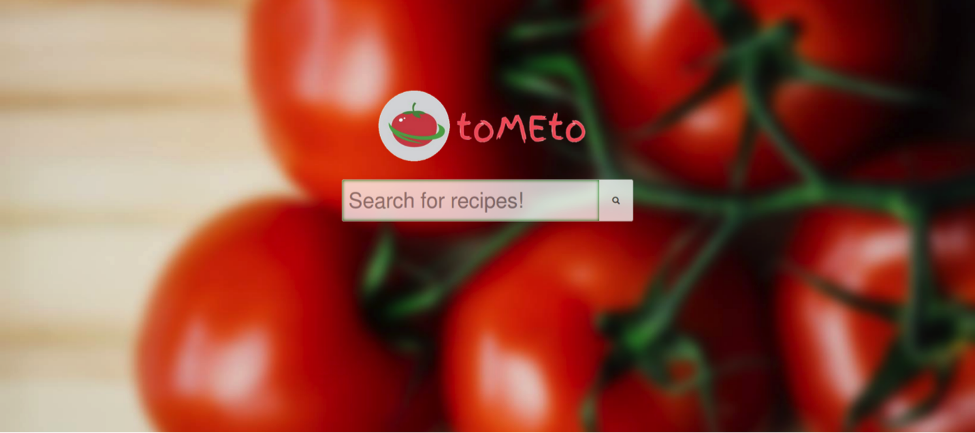
\includegraphics[width=.95\textwidth]{p1.png}
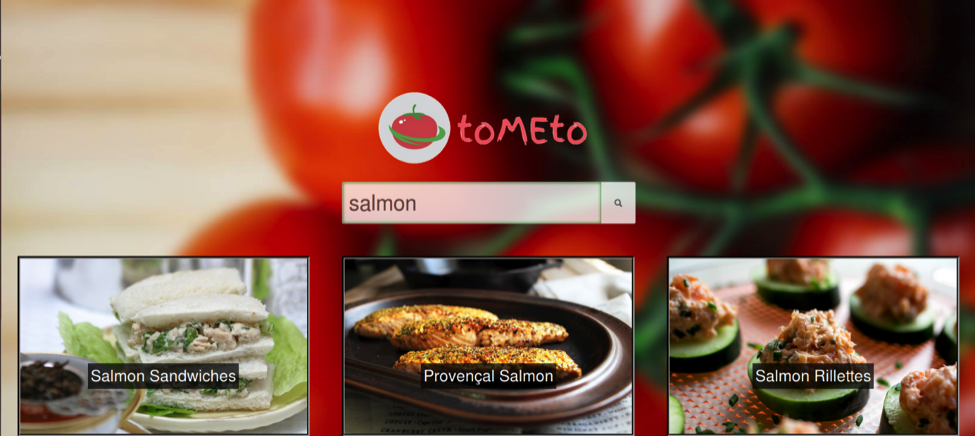
\includegraphics[width=.95\textwidth]{p2.png}
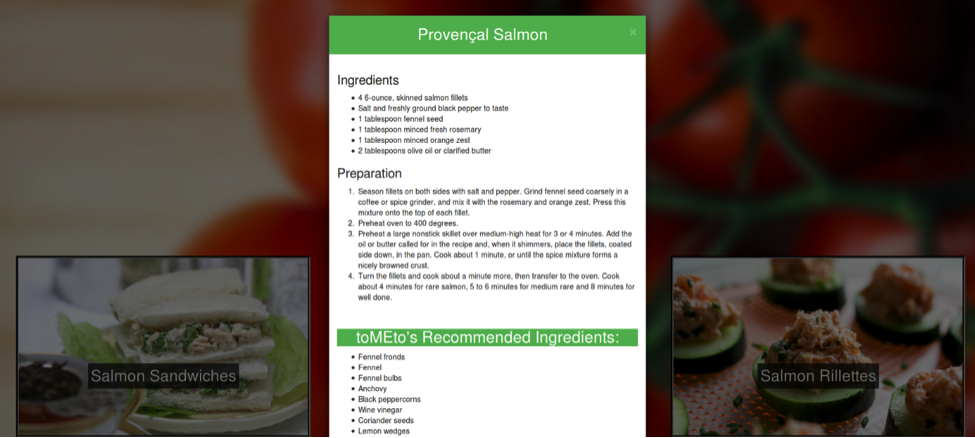
\includegraphics[width=.95\textwidth]{p3.png}
\end{figure}

\clearpage
\onecolumn
\section*{Appendix B: Software Architecture}
\vspace{3mm} %3mm vertical space

\begin{table}[h]
       \begin{tabular}{ | l | l | p{5cm} |}
       \hline
       Directory & Contains & Notable files \\ 
       \hline
       \texttt{src/} & Root of toMEto source code & \texttt{app.py} \\ \hline
       \texttt{src/static} & Images, CSS, JavaScript used by the frontend (Flask) & \\ \hline
       \texttt{src/templates} & HTML templates used by the frontend (Flask) & \\ \hline
       \texttt{src/backend} & Backend scripts & \texttt{algorithm\_analyzer.py} \\
                            &                 & \texttt{search.py} \\ \hline
       \texttt{src/backend/data} & Data processing & \texttt{allrecipes\_mapper.py} \\
                                 &                 & \texttt{allrecipes\_parser.py} \\
                                 &                 & \texttt{nyt\_mapper.py}  \\
                                 &                 & \texttt{nyt\_parser.py} \\ 
                                 &                 & \texttt{scraper.py} \\ \hline
       \texttt{src/backend/analyzers} & Different recommendation algorithms & \texttt{analyzer\_*.py} \\
                                      &                                     & \texttt{utils.py} \\ \hline
       \end{tabular}
       \caption{Source code organization}
\end{table}

\begin{table}[h]
    \centering
    \begin{tabular}{ | p{5cm} | p{2cm} | p{2cm} | p{1cm} | p{6cm} |}
    \hline
    Module Name & Language & Author & Lines of Code & Description/Functionality \\  \hline
    \texttt{data/scraper.py} & Python & Charlie & ~100 & Scrapes for recipes off NYT and Allrecipes websites \\ \hline
    \texttt{data/allrecipes\_parser.py},
    \texttt{data/nyt\_parser.py} & Python & Charlie & ~150 & Extracts relevant information (title, ingredients, body) from scraped recipes \\ \hline
    \texttt{data/allrecipes\_mapper.py},
    \texttt{data/nyt\_mapper.py} & Python & Charlie & ~400 & Finds top ingredients and maps uncommon ingredients to real ones (improves data quality) \\ \hline
    \texttt{analyzers/analyzer\_*.py} & Python & Charlie, Matthew, Albert & ~600 & Different algorithms for recommendations \\ \hline
    \texttt{analyzers/utils.py} & Python & Charlie, Matthew, Albert & ~200 & Utility functions used by different files \\ \hline
    \texttt{backend/algorithm\_analyzer.py} & Python & Matthew, Albert & ~200 & Objectively tests differences between algorithms \\ \hline
    \texttt{backend/search.py} & Python & Matthew & ~20 & Handles user search queries (forward to NYT search) \\ \hline
    \texttt{src/app.py} and CSS/HTML & Python/Flask, CSS, HTML, Javascript & Jonathan & ~600 & Entry point to the program, used to start up the toMEto service (built using Flask Framework) \\ \hline
    \end{tabular}
    \caption{List of modules used in toMEto.}
\end{table}

\end{document}
